\documentclass[a4paper,14pt, unknownkeysallowed]{extreport}

\usepackage{cmap} % Улучшенный поиск русских слов в полученном pdf-файле
\usepackage[T2A]{fontenc} % Поддержка русских букв
\usepackage[utf8]{inputenc} % Кодировка utf8
\usepackage[english,russian]{babel} % Языки: русский, английский
\usepackage{enumitem}

 
\usepackage{threeparttable}

\usepackage[14pt]{extsizes}

\usepackage{caption}
\captionsetup{labelsep=endash}
\captionsetup[figure]{name={Рисунок}}

% \usepackage{ctable}
% \captionsetup[table]{justification=raggedleft,singlelinecheck=off}

\usepackage{amsmath}

\usepackage{geometry}
\geometry{left=30mm}
\geometry{right=10mm}
\geometry{top=20mm}
\geometry{bottom=20mm}

\usepackage{titlesec}
\titleformat{\section}
	{\normalsize\bfseries}
	{\thesection}
	{1em}{}
\titlespacing*{\chapter}{0pt}{-30pt}{8pt}
\titlespacing*{\section}{\parindent}{*4}{*4}
\titlespacing*{\subsection}{\parindent}{*4}{*4}

\usepackage{setspace}
\onehalfspacing % Полуторный интервал

\frenchspacing
\usepackage{indentfirst} % Красная строка

\usepackage{titlesec}
\titleformat{\chapter}{\LARGE\bfseries}{\thechapter}{20pt}{\LARGE\bfseries}
\titleformat{\section}{\Large\bfseries}{\thesection}{20pt}{\Large\bfseries}

\usepackage{multirow}
\usepackage{listings}
\usepackage{xcolor}

% Для листинга кода:
\lstset{%
	language=Matlab,   					% выбор языка для подсветки	
	basicstyle=\small\sffamily,			% размер и начертание шрифта для подсветки кода
	numbers=left,						% где поставить нумерацию строк (слева\справа)
	numberstyle=\tiny,		     		% размер шрифта для номеров строк
	stepnumber=1,						% размер шага между двумя номерами строк
	numbersep=5pt,						% как далеко отстоят номера строк от подсвечиваемого кода
	frame=single,						% рисовать рамку вокруг кода
	tabsize=4,							% размер табуляции по умолчанию равен 4 пробелам
	captionpos=t,						% позиция заголовка вверху [t] или внизу [b]
	breaklines=true,					
	breakatwhitespace=true,				% переносить строки только если есть пробел
	backgroundcolor=\color{white},
	basicstyle=\footnotesize\ttfamily,
	keywordstyle=\color{blue},
	stringstyle=\color{red},
	commentstyle=\color{gray},
	showspaces=false,
    showstringspaces=false
}


\usepackage{pgfplots}
\usetikzlibrary{datavisualization}
\usetikzlibrary{datavisualization.formats.functions}


\lstset{
	literate=
	{а}{{\selectfont\char224}}1
	{б}{{\selectfont\char225}}1
	{в}{{\selectfont\char226}}1
	{г}{{\selectfont\char227}}1
	{д}{{\selectfont\char228}}1
	{е}{{\selectfont\char229}}1
	{ж}{{\selectfont\char230}}1
	{з}{{\selectfont\char231}}1
	{и}{{\selectfont\char232}}1
	{й}{{\selectfont\char233}}1
	{к}{{\selectfont\char234}}1
	{л}{{\selectfont\char235}}1
	{м}{{\selectfont\char236}}1
	{н}{{\selectfont\char237}}1
	{о}{{\selectfont\char238}}1
	{п}{{\selectfont\char239}}1
	{р}{{\selectfont\char240}}1
	{с}{{\selectfont\char241}}1
	{т}{{\selectfont\char242}}1
	{у}{{\selectfont\char243}}1
	{ф}{{\selectfont\char244}}1
	{х}{{\selectfont\char245}}1
	{ц}{{\selectfont\char246}}1
	{ч}{{\selectfont\char247}}1
	{ш}{{\selectfont\char248}}1
	{щ}{{\selectfont\char249}}1
	{ъ}{{\selectfont\char250}}1
	{ы}{{\selectfont\char251}}1
	{ь}{{\selectfont\char252}}1
	{э}{{\selectfont\char253}}1
	{ю}{{\selectfont\char254}}1
	{я}{{\selectfont\char255}}1
	{А}{{\selectfont\char192}}1
	{Б}{{\selectfont\char193}}1
	{В}{{\selectfont\char194}}1
	{Г}{{\selectfont\char195}}1
	{Д}{{\selectfont\char196}}1
	{Е}{{\selectfont\char197}}1
	{Ж}{{\selectfont\char198}}1
	{З}{{\selectfont\char199}}1
	{И}{{\selectfont\char200}}1
	{Й}{{\selectfont\char201}}1
	{К}{{\selectfont\char202}}1
	{Л}{{\selectfont\char203}}1
	{М}{{\selectfont\char204}}1
	{Н}{{\selectfont\char205}}1
	{О}{{\selectfont\char206}}1
	{П}{{\selectfont\char207}}1
	{Р}{{\selectfont\char208}}1
	{С}{{\selectfont\char209}}1
	{Т}{{\selectfont\char210}}1
	{У}{{\selectfont\char211}}1
	{Ф}{{\selectfont\char212}}1
	{Х}{{\selectfont\char213}}1
	{Ц}{{\selectfont\char214}}1
	{Ч}{{\selectfont\char215}}1
	{Ш}{{\selectfont\char216}}1
	{Щ}{{\selectfont\char217}}1
	{Ъ}{{\selectfont\char218}}1
	{Ы}{{\selectfont\char219}}1
	{Ь}{{\selectfont\char220}}1
	{Э}{{\selectfont\char221}}1
	{Ю}{{\selectfont\char222}}1
	{Я}{{\selectfont\char223}}1
}

\usepackage{graphicx}
\newcommand{\img}[3] {
	\begin{figure}[h!]
		\center{\includegraphics[height=#1]{img/#2}}
		\caption{#3}
		\label{img:#2}
	\end{figure}
}


\usepackage[justification=centering]{caption} % Настройка подписей float объектов

\usepackage[unicode,pdftex]{hyperref} % Ссылки в pdf
\hypersetup{hidelinks}

\usepackage{csvsimple}

\newcommand{\code}[1]{\texttt{#1}}

\usepackage{longtable}

\usepackage{array}
\usepackage{booktabs}
\usepackage{floatrow}

\floatsetup[longtable]{LTcapwidth=table}

% \def\UrlBreaks{\do\/\do-\do\_}

\makeatletter
\renewcommand*\l@chapter[2]{%
  \ifnum \c@tocdepth >\m@ne
    \addpenalty{-\@highpenalty}%
    \vskip 1.0em \@plus\p@
    \setlength\@tempdima{1.5em}%
    \begingroup
      \parindent \z@ \rightskip \@pnumwidth
      \parfillskip -\@pnumwidth
      \leavevmode \bfseries
      \advance\leftskip\@tempdima
      \hskip -\leftskip
      #1\nobreak\normalfont\leaders\hbox{$\m@th
        \mkern \@dotsep mu\hbox{.}\mkern \@dotsep
        mu$}\hfill\nobreak\hb@xt@\@pnumwidth{\hss #2}\par
      \penalty\@highpenalty
    \endgroup
  \fi}
\makeatother

\begin{document}



\begin{titlepage}
	\newgeometry{pdftex, left=2cm, right=2cm, top=2.5cm, bottom=2.5cm}
	\fontsize{12pt}{12pt}\selectfont
	\noindent \begin{minipage}{0.15\textwidth}
		
\includegraphics[width=\linewidth]{img/b_logo.jpg}
	\end{minipage}
	\noindent\begin{minipage}{0.9\textwidth}\centering
		\textbf{Министерство науки и высшего образования Российской Федерации}\\
		\textbf{Федеральное государственное бюджетное образовательное учреждение высшего образования}\\
		\textbf{«Московский государственный технический университет имени Н. Э.~Баумана}\\
		\textbf{(национальный исследовательский университет)»}\\
		\textbf{(МГТУ им. Н. Э.~Баумана)}
	\end{minipage}
	
	\noindent\rule{18cm}{3pt}
	\newline\newline
	\noindent ФАКУЛЬТЕТ $\underline{\text{«Информатика и системы управления»~~~~~~~~~~~~~~~~~~~~~~~~~~~~~~~~~~~~~~~~~~~~~~~~~~~~~~~}}$ \newline\newline
	\noindent КАФЕДРА $\underline{\text{«Программное обеспечение ЭВМ и информационные технологии»~~~~~~~~~~~~~~~~~~~~~~~}}$\newline\newline\newline\newline\newline\newline\newline
	
	
	\begin{center}
		\noindent\begin{minipage}{1.3\textwidth}\centering
		\Large\textbf{   ~~~ Лабораторная работа №1}\newline
		\textbf{по курсу "Математическая статистика"}\newline\newline\newline\newline
		\end{minipage}
	\end{center}
	
	\noindent\textbf{Тема} 			$\underline{\text{Гистограмма и эмпирическая функция распределения}}$\newline\newline
	\noindent\textbf{Студент} 		$\underline{\text{Ковалец К. Э.~~~~~~~~~~~~~~~~~~~~~~~~~~~~~~~~~~~~~~~~~~~~~~~~~~}}$\newline\newline
	\noindent\textbf{Группа} 		$\underline{\text{ИУ7-63Б~~~~~~~~~~~~~~~~~~~~~~~~~~~~~~~~~~~~~~~~~~~~~~~~~~~~~~~~~~~}}$\newline\newline
	\noindent\textbf{Вариант} 		$\underline{\text{9~~~~~~~~~~~~~~~~~~~~~~~~~~~~~~~~~~~~~~~~~~~~~~~~~~~~~~~~~~~~~~~~~~~~}}$\newline\newline
	\noindent\textbf{Преподаватель} $\underline{\text{Власов П. А.~~~~~~~~~~~~~~~~~~~~~~~~~~~~~~~~~~~~~~~~~}}$\newline
	
	\begin{center}
		\vfill
		Москва~---~\the\year
		~г.
	\end{center}
	\restoregeometry
\end{titlepage}



\setcounter{page}{2}

\chapter{Содержание работы}

\begin{enumerate}
    \item Для выборки объема \textit{n} из генеральной совокупности \textit{X} реализовать в виде программы на ЭВМ

    \begin{itemize}
        \item вычисление максимального значения $M_{max}$ и минимального значения $M_{min}$;
        \item размаха $R$ выборки;
        \item вычисление оценок $\hat\mu$ и $S^2$ математического ожидания $MX$ и дисперсии $DX$;
        \item группировку значений выборки в $m = [\log_2 n] + 2$ интервала;
        \item построение на одной координатной плоскости гистограммы и графика функции плотности распределения вероятностей нормальной случайной величины с математическим ожиданием $\hat{\mu}$ и дисперсией $S^2$;
        \item построение на другой координатной плоскости графика эмпирической функции распределения и функции распределения нормальной случайной величины с математическим ожиданием $\hat{\mu}$ и дисперсией $S^2$.
    \end{itemize}

    \item Провести вычисления и построить графики для выборки из индивидуального варианта.
\end{enumerate}

\chapter{Формулы для вычисления величин}

\begin{itemize}

	\item Максимальное $M_{max}$ значение выборки:

	\begin{equation}
		\begin{aligned}
			M_{\max} = X_{(n)}
		\end{aligned}
	\end{equation}

	\item Минимальное $M_{min}$ значение выборки:

	\begin{equation}
		\begin{aligned}
			M_{\min} = X_{(1)}
		\end{aligned}
	\end{equation}

	\item Размах $R$ выборки:

	\begin{equation}
		R = M_{\max} - M_{\min}
	\end{equation}

    \item Выборочное среднее (оценка математического ожидания):

    \begin{equation}
        \begin{aligned}
        \hat\mu(\vec X_n) &= \frac 1n \sum_{i=1}^n X_i\\
        \end{aligned}
    \end{equation}
    
    \item Исправленная выборочная дисперсия:

    \begin{equation}
        \begin{aligned}
        S^2(\vec X_n) &= \frac 1{n-1} \sum_{i=1}^n (X_i-\overline X_n)^2
        \end{aligned}
    \end{equation}

\end{itemize}


\chapter{Определение эмпирической плотности, гистограммы и эмпирической функции распределения}

Если объем выборки достаточно велик ($n > 50$), то элементы выборки группируются в так называемый статистический ряд. Для этого отрезок\newline $J = [x_{(1)}, x_{(n)}]$ разбивают на $m$ равновеликих промежутков.\newline

Ширина каждого из них:

\begin{equation}
    \Delta = \frac{|J|}{m} = \frac{x_{(n)} - x_{(1)}}{m},
\end{equation}

где $m = [\log_2 n] + 2$, $x_{(1)} = min(\vec x)$, $x_{(n)} = max(\vec x)$.\newline

Далее полагают $m$:

\begin{equation}
    J_i = [x_{(1)} + (i - 1) \cdot \Delta, x_{(1)} + i \cdot \Delta), i = \overline{1; m - 1}
\end{equation}

\begin{equation}
    J_{m} = [x_{(1)} + (m - 1) \cdot \Delta, x_{(n)}]
\end{equation}

\section{Интервальный статистический ряд}

\textbf{Опр.} Интервальным статистическим рядом, отвечающим выборке $\vec x$, называется таблица вида:

\begin{table}[htb]
    \centering
    \begin{tabular}{|c|c|c|c|c|}
        \hline
        $J_1$ & $J_2$ & ... & $J_m$ \\
        \hline
        $n_1$ & $n_2$ & ... & $n_m$ \\
        \hline
    \end{tabular}
\end{table}

Здесь $n_i$ --- число элементоав выборки $\vec x$, попавших в промежуток $J_i$, $i$ = $\overline{1, m}$.

\clearpage

\section{Эмпирическая плотность}

Пусть для данной выборки $\vec x$ построен интервальный статистический ряд $(J_i, n_i)$, $i = \overline{1; m}$\newline

\textbf{Опр.} Эмпирической плотностью распределния (соответствующей выборке $\vec x$) называется функция:

\begin{equation}
    f_n(x) =
    \begin{cases}
        \frac{n_i}{n \cdot \Delta}, x \in J_i, i = \overline{1; m} \\
        0, \text{иначе} \\
    \end{cases}
\end{equation}


\section{Гистограмма}

\textbf{Опр.} График эмпирической функции плотности называется гистограммой.


\section{Эмпирическая функция распределения}

Пусть $\vec x = (x_1, ..., x_n)$ --- выборка из генеральной совокупности $X$.

Обозначим $n(t, \vec x)$ --- число компонент вектора $\vec x$, которые меньше, чем $t$.\newline

\textbf{Опр.} Эмпирической функцией распределения, построенной по выборке $\vec x$, называют функцию

\begin{equation}
    F_n: {R} \to {R},
\end{equation}

определенную правилом:

\begin{equation}
    F_n(x) = \frac{n(t, \vec x)}{n}.
\end{equation}

\chapter{Текст программы}

\lstinputlisting{../src/lab_1.m}

\chapter{Результат работы программы}

\begin{figure}[h]
	\centering
	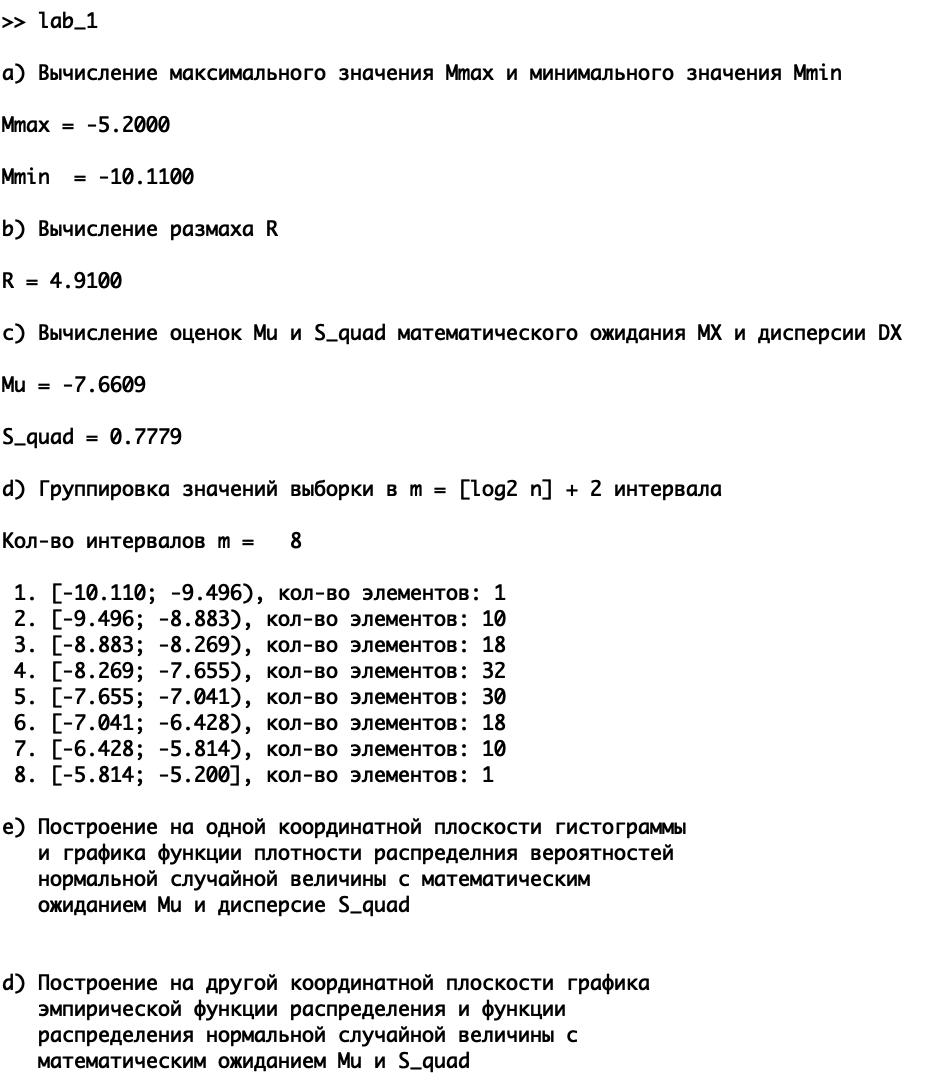
\includegraphics[scale=0.95]{img/result.png}
	\caption{Результаты расчетов для выборки из индивидуального варианта}
	\label{fig:result}
\end{figure}

\begin{figure}[h]
	\centering
	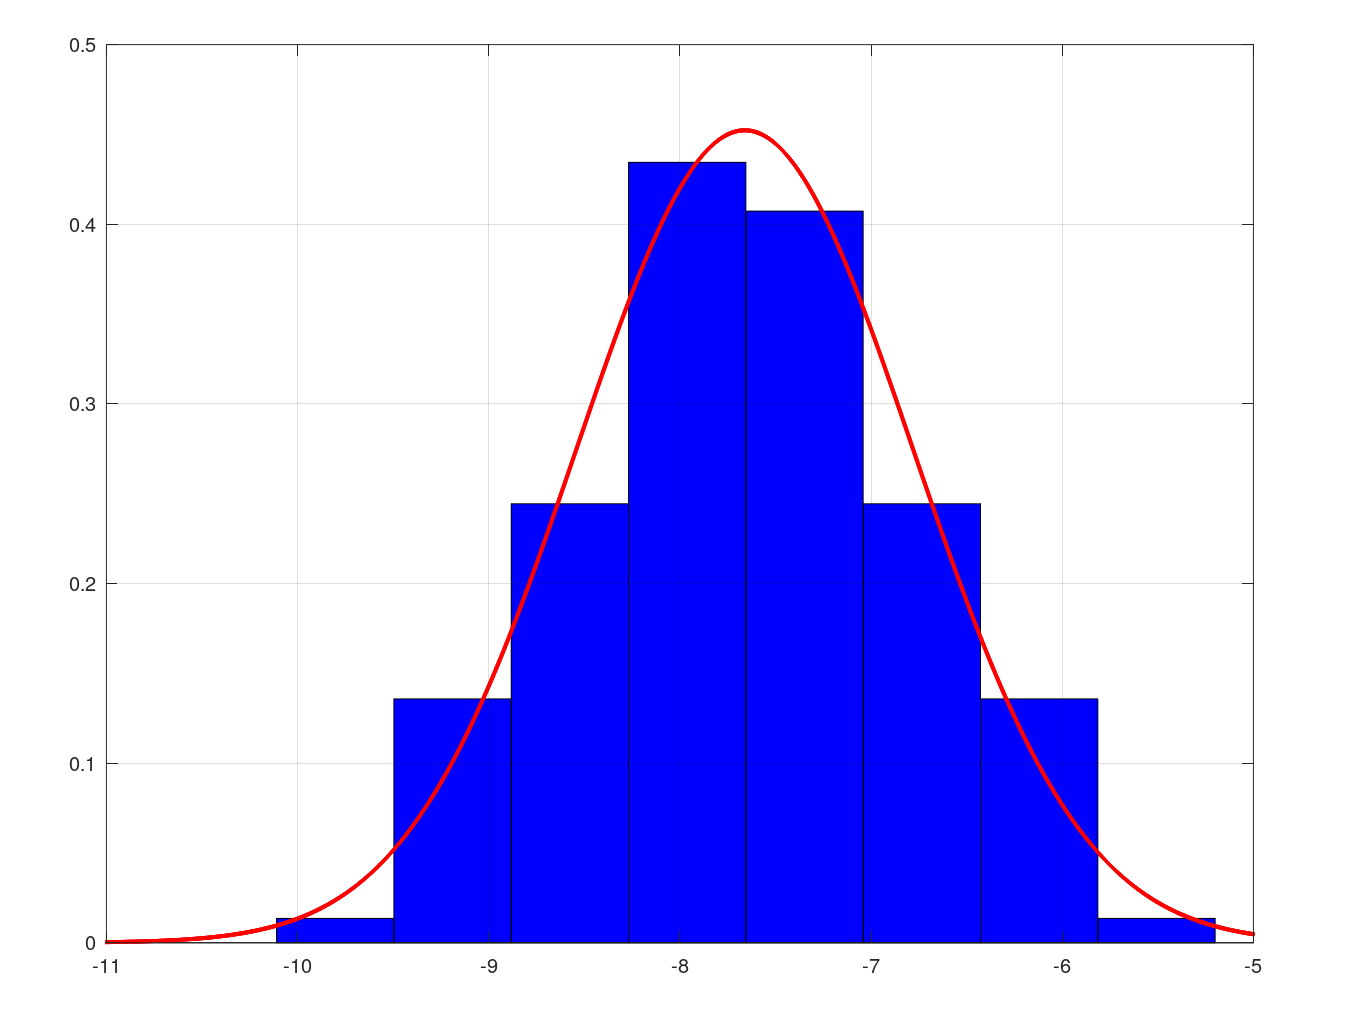
\includegraphics[scale=0.5]{img/histo.png}
	\caption{Гистограмма и график функции плотности распределения нормальной случайной величины с выборочными математическим ожиданием и дисперсией}
	\label{fig:histo}
\end{figure}

\begin{figure}[h]
	\centering
	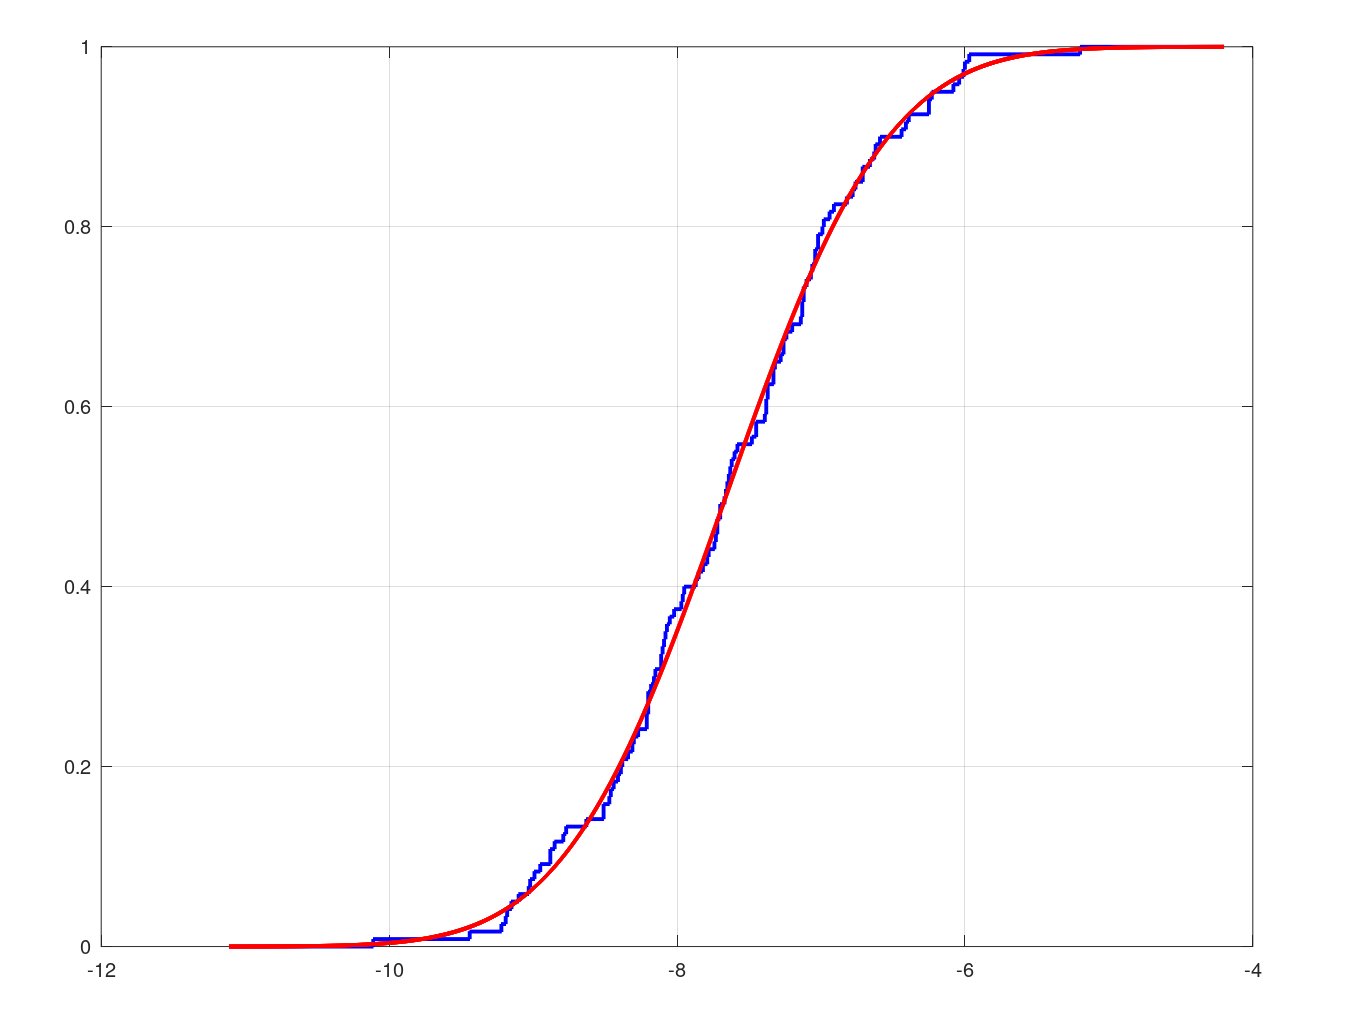
\includegraphics[scale=0.5]{img/emperic.png}
	\caption{График эмперической функции распределения и функции распределения нормальной случайной величины с выборочными математическим ожиданием и дисперсией}
	\label{fig:emperic}
\end{figure}

\end{document}
